% Online Learning: Static vs Pure Incremental vs Hybrid
% Replaces: tab:online-learning-corrected + tab:hybrid-results in section_online_learning_validation.tex
% Grouped bar chart showing the breakthrough hybrid solution

\begin{figure}[htbp]
\centering
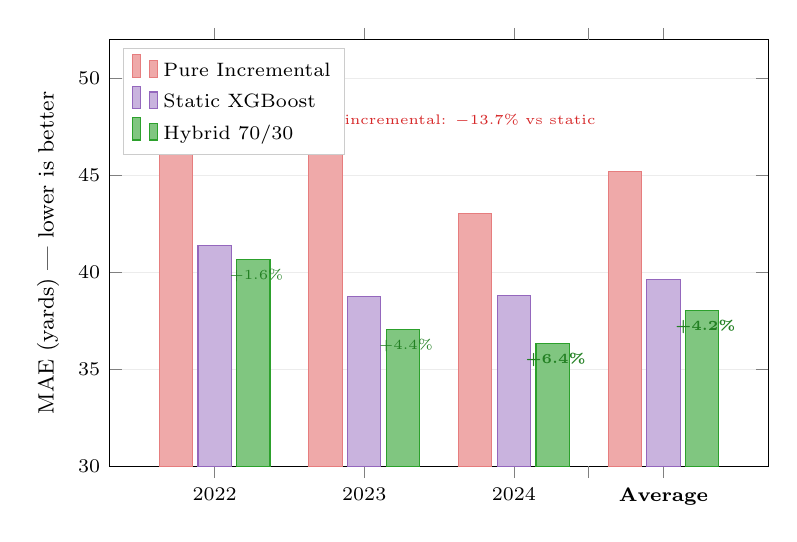
\begin{tikzpicture}
\definecolor{colStatic}{RGB}{148,103,189}
\definecolor{colIncr}{RGB}{214,39,40}
\definecolor{colHybrid}{RGB}{44,160,44}

\begin{axis}[
  width=0.82\textwidth,
  height=7cm,
  ybar,
  bar width=12pt,
  ylabel={MAE (yards) --- lower is better},
  ylabel style={font=\footnotesize},
  ymin=30, ymax=52,
  xtick={1,2,3,4},
  xticklabels={2022, 2023, 2024, {\textbf{Average}}},
  xticklabel style={font=\scriptsize},
  yticklabel style={font=\scriptsize},
  legend style={at={(0.02,0.98)}, anchor=north west, font=\scriptsize, draw=gray!40, cells={anchor=west}},
  grid=major,
  grid style={gray!15},
  xmajorgrids=false,
  enlarge x limits={abs=0.7},
  extra x ticks={3.5},
  extra x tick labels={},
  extra x tick style={grid style={black!25, dashed}},
]

% Incremental bars (worst)
\addplot[fill=colIncr!40, draw=colIncr!60] coordinates {
  (1, 46.26) (2, 46.39) (3, 43.02) (4, 45.22)
};
\addlegendentry{Pure Incremental}

% Static bars
\addplot[fill=colStatic!50, draw=colStatic] coordinates {
  (1, 41.37) (2, 38.78) (3, 38.82) (4, 39.66)
};
\addlegendentry{Static XGBoost}

% Hybrid bars (best)
\addplot[fill=colHybrid!60, draw=colHybrid] coordinates {
  (1, 40.69) (2, 37.07) (3, 36.33) (4, 38.03)
};
\addlegendentry{Hybrid 70/30}

% Improvement trend for hybrid
\node[font=\tiny, text=colHybrid!80!black, anchor=north] at (axis cs:1.28,40.69) {+1.6\%};
\node[font=\tiny, text=colHybrid!80!black, anchor=north] at (axis cs:2.28,37.07) {+4.4\%};
\node[font=\tiny\bfseries, text=colHybrid!80!black, anchor=north] at (axis cs:3.28,36.33) {+6.4\%};
\node[font=\tiny\bfseries, text=colHybrid!80!black, anchor=north] at (axis cs:4.28,38.03) {\textbf{+4.2\%}};

% Failure annotation for incremental
\node[font=\tiny, text=colIncr, anchor=south west, align=left] at (axis cs:1.5,47)
  {Pure incremental: $-$13.7\% vs static};

\end{axis}
\end{tikzpicture}
\caption[Online learning: static vs hybrid]{Online learning validation (2022--2024). Pure incremental XGBoost underperforms static by 13.7\%, but the 70/30 hybrid blend achieves +4.2\% improvement with increasing gains across seasons (+1.6\% $\to$ +4.4\% $\to$ +6.4\%). The hybrid captures mid-season adaptation without sacrificing baseline stability.}
\label{fig:hybrid-online-chart}
\end{figure}
